%!TEX root = ../main.tex
\chapter{Introduction}
\label{chap:introduction}
This chapter begins by introducing the issue to be addressed throughout the present dissertation, stating the current situation and analyse it from the perspective of existing solutions. The following section outlines the project rationale and presents the intended outcomes. The next section states the objectives and relationship between them, after which it details the method of critically evaluating the project's success criteria. The penultimate section describes the risk analysis performed and the proactive actions designed to mitigate the identified risks. Finally, the last section presents an overview of the remaining chapters of the dissertation.

\begin{figure}[b]
	\centering
	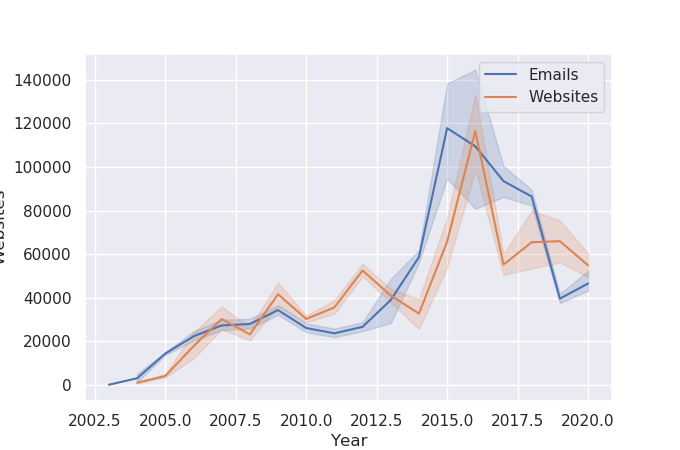
\includegraphics[width=0.49\textwidth]{apwg_attack_hist.png}
	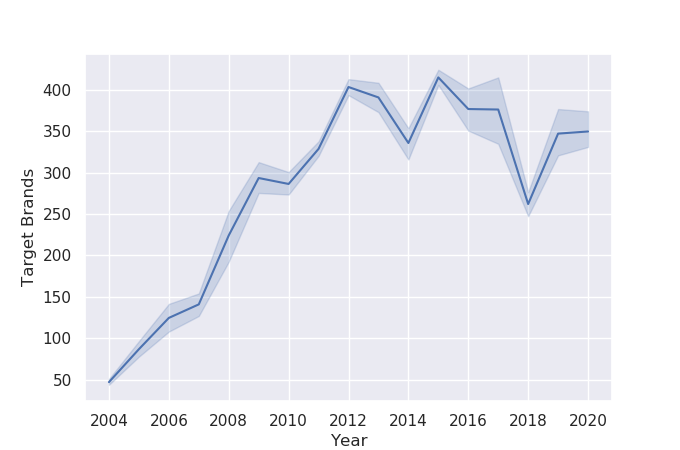
\includegraphics[width=0.49\textwidth]{apwg_brands_hist.png}
	\caption{A high-level illustration of phishing attacks over the years \citep{APWG}}
	\label{fig:PHISHING_HISTORY}
\end{figure}

\section{Problem definition}
\label{sec:problem_definition}
While the exploitation of trust or personality traits such as agreeableness or obedience is not a new phenomenon, the internet has brought about a new framework in which such activities can be conducted. Comparing those as mentioned earlier to a face-to-face setting, the former provides several advantages for the attacker, such as anonymity and a greater geographical reach. Once with this contextual shift, the term "phishing" has been popularised. Phishing is described as a scam by which an internet user is manipulated into disclosing personal or confidential information that the attacker can use illicitly \citep{Merriam_Webster}.

In its primitive form, a phishing attack requires elementary technical knowledge. The main skills required are the ones easily transferable from manipulation or deceit in face-to-face interaction. This factor, amongst other outlined in the following chapter, have contributed to the popularity growth of phishing attacks in the past twenty-five years.

\subsection{Current situation}
\label{subsec:current_situation}
The gain in popularity is reflected in the numbers registered by the Anti-Phishing Working Group \citep{APWG}. Their archives open with the reports from across 2004. These add up to 33.5 thousand unique registered phishing attacks with missing data for September. After fifteen years, the APWG registered 479,468 unique phishing attacks in 2019. Besides the growth in numbers, these reports outline a clear advancement in the technical aspects of registered phishing campaigns as well. One example of this is the adoption of Transport Layer Security (TLS) used to serve phishing websites over Hypertext Transfer Protocol Secure (HTTPS). Reported usage had grown from close to 0\% in 2016, to 68\% by the end of the third quarter of 2019 \citep{APWG_Q42019}.

\subsection{Existing solutions}
\label{subsec:existing_solutions}
In most cases, the only source of protection against accessing phishing websites
the user has is the browser. Browser usage statistics show that Google
Chrome, Apple Safari, and Mozilla Firefox comprise 86.59\% \citep{Statcounter} of the market share. All of these browsers use Google Safe Browsing (GSB) as their anti-phishing detection system. At the surface level, this is a blacklist based service which provides the aforementioned browsers with a list of malicious Uniform Resource Locators (URL) through its
Application Programming Interface (API).

\begin{figure}[t]
	\centering
	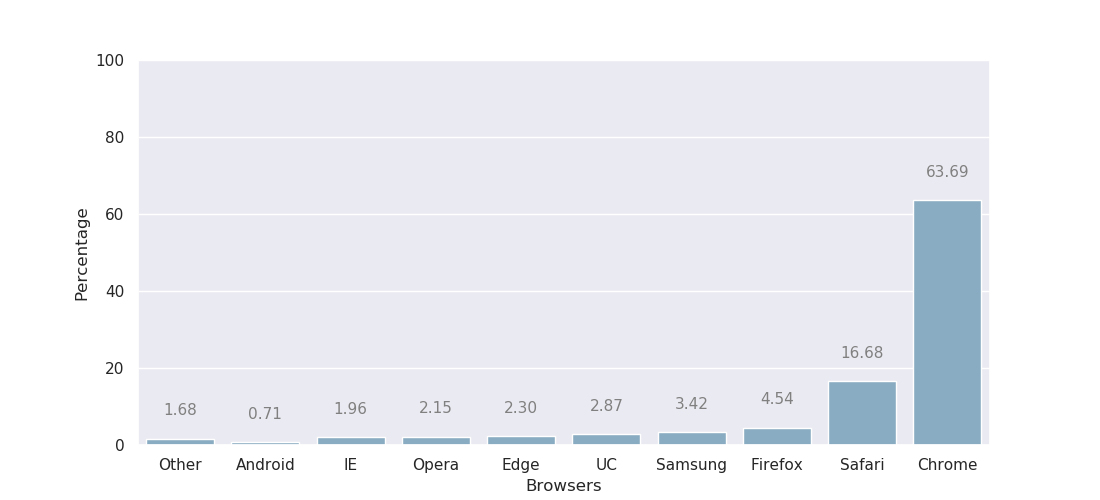
\includegraphics[width=0.90\textwidth]{browser_marketshare.png}
	\caption{Browser market share \citep{Statcounter}}
	\label{fig:BROWSER_MARKETSHARE}
\end{figure}

Although GSB acts as a blacklist, underneath this compilation of malicious URLs lies an entire process of scrutinisation. Based on it, the decision-making mechanism chooses whether the URL of the studied web page should be added to the blacklist. Classification efficiency aside, the time needed for this process to finalise and update the list renders the solution suboptimal. The core issue is that malicious actors are quick in conducting these attacks, which makes them go under GSB's radar. Given that the reported median phishing webpage lifespan is of less than twenty-four hours \citep{Kelly_Sheridan}, speed is a crucial factor in defending against them.

Another anti-phishing detection system worth mentioning is Microsoft SmartScreen. SmartScreen is embedded in the Windows operating system and delivers protection against a wide range of threats. Phishing protection is offered through Microsoft's Internet Explorer and Edge browsers which represent 4.25\% of the market share. Although SmartScreen advertises better protection than GSB, the improvement reported by the literature is of 2.6\% \citep{Adebowale}. One significant mention is that all analysis is done off-site, thus plenty of information has to be sent to Microsoft's servers for processing. Depending on the circumstances, doing so might have an impact on privacy.

In conclusion, the user's central defence against phishing is not versatile or agile enough to keep up with the speed and sophistication of these attacks.


\section{Project rationale and outcomes}
\label{sec:project_rationale_and_outcomes}
The trends and statistics outline the fact that phishing will remain a prevalent type of attack for the foreseeable future. Still, the protection mechanisms of the main medium of interaction with phishing webpages are not satisfactory, as shown by the amount of financial damage reported every year \citep{APWG_Q42019}. Furthermore, identity theft is difficult to recover from as it takes time and discipline.

Given the shortage of empirical evaluations of GSB's protection, this dissertation sets to investigate its prediction accuracy. This evaluation, in addition to further research, serves as baseline performance for the artefact. The solution aims to stack elements extracted from the corroboration of literature and experiment with new approaches as well. The final implementation aims to outperform GSB while acknowledging the circumstances and priorities of such a system.

To the best of my knowledge, there is no other approach structured as specified above, which comprises the motivation of the project. There are not many iterations of anti-phishing detection systems either aiming to outperform GSB or target users with reduced technical literacy.


\section{Aim and objectives}
\subsection{Aim}
\label{subsec:aim}
The intended functional outcome of the project is a piece of software that addresses the previously articulated arguments against GSB. The first step in doing so is to develop the means to evaluate its efficiency. The second step is composed of research, design, and development of an improved solution.

\begin{landscape}
	\begin{singlespace}
		\subsection{Objectives}
		\begin{center}
			\label{tab:OBJECTIVES}
			\begin{tabular}{ | m{0.5em} | m{18.5em} | m{23em}| m{16em} | }
				\hline
				\textbf{\#} & \textbf{Objective} & \textbf{Objective actions} &
				\textbf{Success criteria}                                                                                                                                  \\
				\hline
				\textbf{1}  &
				To research and develop a mechanism for evaluating the
				accuracy of the phishing detection system embedded in popular
				browsers (Google Safe Browsing).
				            &
				1. Research how Google Safe Browsing works and possible methods of evaluation.		\newline\newline
				2. Find the appropriate tools and libraries to automate the
				process of evaluation.
				\newline\newline
				2. Enter a design, development and evaluation cycle until the
				automation script proves to be reliable.
				            &
				The final product evaluates the phishing detection system of
				browsers with a minimal error margin.                                                                                                                      \\


				\hline
				\textbf{2}  &
				To research and bring together different anti-phishing methods
				described in the literature into an effective phishing
				detection design.
				            &
				1. Research different approaches towards phishing detection
				systems.
				\newline\newline
				2. Build a creative selection of features and design the high-level overview of the system to be implemented.
				            &
				The final design resembles well established anti-phishing detection systems to ensure the foundation of experimentation is proven solid by the literature. \\


				\hline
				\textbf{3}  &
				To implement and optimise a solution that improves the status quo and can be operated with minimal technical literacy. The implementation should also consider the intended operational environment and its particularities.
				            &
				1. Research the value of a whitelist approach to save resources consumed by machine learning model predictions.
				\newline\newline
				2. Train the machine learning models and review its classification accuracy.
				\newline\newline
				3. Evaluate the model and calibrate it to fit the intended operational environment while delivering satisfactory classification accuracy.
				            &
				The solution developed either surpasses or complements Google Safe Browsing in achieving a better classification accuracy.                                 \\

				\hline
			\end{tabular}
			\captionsetup{type=table}\caption{Objectives list}
		\end{center}
	\end{singlespace}
\end{landscape}
\section{Risk Analysis}

Considering the nature of this dissertation and the extensive amount it plans to achieve, a risk analysis is a useful resource. It will assure a proactive stance regarding the obstacles that might be encountered. Besides the resilience it offers, it helps in acknowledging areas where problems may arise and prioritise work items based on this.

Table \ref{tab:RISK_ANALYSIS} presents the main identified risks related to this project. Each of these has a likelihood and impact metric attributed to better outline the hierarchy of prioritisation.

\begin{singlespace}
	\begin{center}
		\label{tab:RISK_ANALYSIS}
		\begin{tabular}{ | m{0.5em} | m{7em} | m{5em} | m{3.2em}| m{17.5em} | }
			\hline
			\textbf{\#} & \textbf{Description} & \textbf{Likelihood} & \textbf{Impact} & \textbf{Intended mitigation}                                                                                                                                \\
			\hline
			\textbf{1}  &
			Time management issues
			            &
			Medium
			            &
			High
			            &
			Develop a plan and Gantt chart before starting the dissertation. Calculate the amount of time necessary to accomplish set objectives and add a sensible error margin to it.                                                              \\
			\hline
			\textbf{2}  &
			Sub-optimal solution results
			            &
			Medium
			            &
			High
			            &

			Allocate more time for the phishing detection system calibration than the estimated necessary. This time ensures that there is enough room for research and experimentation.                                                             \\
			\hline
			\textbf{4}  &
			Inaccurate assumptions
			            &
			High
			            &
			Low
			            &

			Extensive research is conducted at every step of the dissertation. The aim is to avoid presuppositions and ground the work in literature.                                                                                                \\
			\hline
			\textbf{5}  &
			Data loss
			            &
			Low
			            &
			High
			            &
			To address possible data loss, the work carried out complies to the back-up rule of 3-2-1. It dictates that three copies of the data should be stored on at least two mediums of storage, one being off-site.                            \\

			\hline
			\textbf{6}  &
			Chosen tools are not appropriate for the task
			            &
			Low
			            &
			High
			            &
			Do brief or comprehensive background checks for all the tools and
			libraries used in the project depending on their importance to the
			success of the project. At the same time not using more tools or
			libraries than strictly necessary                                                                                                                                                                                                        \\
			\hline

			\textbf{3}  &
			Fatigue, anxiety or health issues
			            &
			Medium
			            &
			High
			            &
			Perform background checks on the tools and libraries used in the project. The amount of research depends on how much the tool influences the fulfilment of set objectives. Furthermore, external resources are used only when necessary. \\
			\hline
		\end{tabular}
		\captionsetup{type=table}\caption{Risk analysis}
	\end{center}
\end{singlespace}

\section{Overview of the dissertation}
\label{sec:overview_of_the_dissertation}
Chapter two explores the relevant literature and introduces previous work done on the subject. Chapter three describes the artefact design and implementation methodology, as well as the evaluation process of both the GSB evaluator and artefact. Chapter four offers an in-depth view of the development process. Furthermore, it follows the process of model calibration and performance enhancement. The fifth chapter compares the solution against GSB and ranks its performance vis-a-vis the literature. The last chapter presents a high-level view of the achievements of this dissertation. It summarises the work conducted and closes with possible ways of further improvement or expansion.